\begin{minipage}{0.55\textwidth}
    \begin{figure}[h]
    \centering
    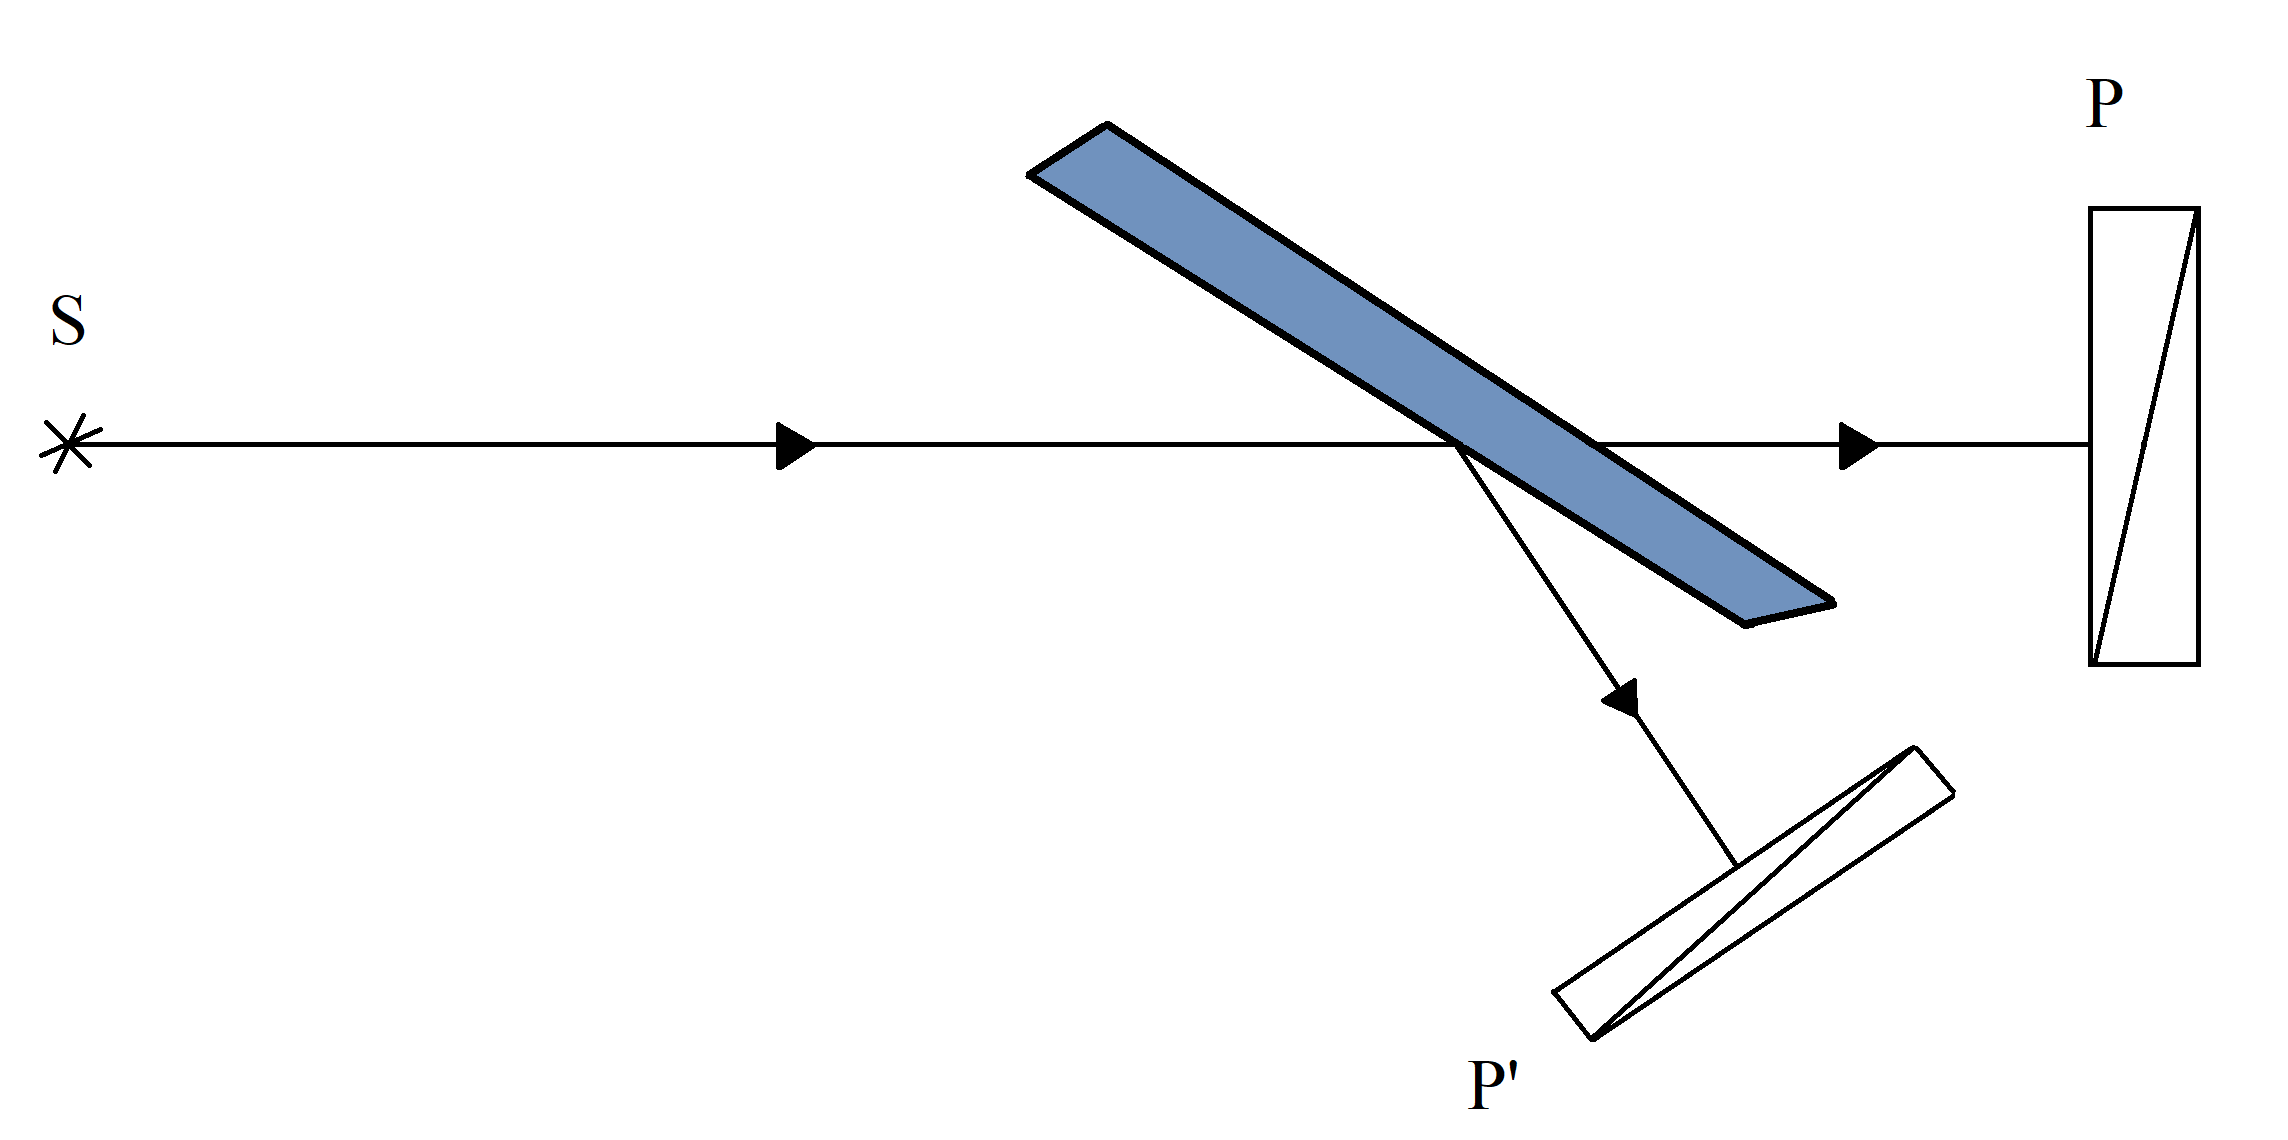
\includegraphics[width=1\textwidth]{images/stoletov.png}
    \caption{The beam goes right to the stack of glass (light blue) and then splits to two polaroids that we investigate before.}
    %\label{fig:}
\end{figure}
\end{minipage}
\hfill
\begin{minipage}{0.35\textwidth}
    So as was expected the reflected and transmitted light had an orthogonal $E$.

    The polaroids are crossed
    \begin{align*}
    	&P_1 \colon 98^\circ&\\
    	&P_2 \colon -265^\circ&
    \end{align*}
\end{minipage}
